\section{Odd Viscosity II}

\subsection{Summary of Last Lecture}
Last time, we explored (in quite a bit of detail) odd viscosity. If we have a linear constitutive equation:
\begin{equation}
    \sigma_{ij} = \eta_{ijkl}v_{kl}
\end{equation}
If this viscosity is derived from entropy production/dissipation $T\dot{S}$, then it must be case that the viscosity tensor is symmetric:
\begin{equation}
    \eta_{ijkl} = \eta_{klij}
\end{equation}
but if we relax this assumption, we can have an odd component:
\begin{equation}
    \eta_{ijkl} = \eta^e_{ijkl} + \eta^o_{ijkl}
\end{equation}
Where the odd part is, as the name suggests, odd under interchange:
\begin{equation}
    \eta^o_{ijkl} = -\eta^o_{klij}
\end{equation}
Note that this part of the tensor cannot be associated with power dissipation. To see this:
\begin{equation}
    P = \eta^o_{ijkl}v_{ij}v_{kl} = \eta^o_{ijkl}v_{kl}v_{ij} = -\eta^o_{klij}v_{kl}v_{ij} = -\eta^o_{ijkl}v_{ij}v_{kl} \implies P = 0
\end{equation}
So, we can see that odd viscosity does not contribute to dissipation, but does contribute to the equation of motion:
\begin{equation}
    \underbrace{D_t v_i}_{\p_t v_i + v_k \p_k v_i} = \p_j \sigma_{ij} + f^{\text{ext}}
\end{equation}
which expanding:
\begin{equation}\label{eq:modNavierStokes}
    \rho D_t v_i = -\p_i p + \eta \Delta v_i + \eta^0\e_{ij}v_j
\end{equation}
possibly supplemented by $\nabla \cdot \v{v} = 0$ if the fluid is incompressible. We can interpret what we have done above as a completion of the Navier-Stokes equation with a chiral term.

\subsection{Odd Viscosity as Pressure}
If we take the above equation and define a new pressure term:
\begin{equation}
    p' = p - \eta^0\omega
\end{equation}
with $\omega$ the vorticity, then we can write:
\begin{equation}
    \rho D_t v_i = -\p_i p' + \eta \Delta v_i
\end{equation}
So the odd viscosity can be reabsorbed into the pressure! Hence we could measure it by measuring the pressure. But if we solved this on a computer, the flow would not change - just a Lagrange multiplier. Hence we call the odd viscosity term a boundary term. Note that the odd viscosity being nothing more than a renormalization of the pressure term is only true if the fluid is incompressible.

The vorticity is the curl of the velocity field:
\begin{equation}
    \gv{\omega} = \nabla \times \v{v}
\end{equation}
or in two dimensions:
\begin{equation}
    \omega = \e_{ij}\p_i v_j = \p_x v_y - \p_y v_x
\end{equation}
Now looking at:
\begin{equation}
    \p_i \omega = \m{\p_x(\p_x v_y - \p_y v_x) \\ \p_y(\p_x v_y - \p_y v_x)}
\end{equation}
The incompressibility condition tells us that:
\begin{equation}
    \p_x v_x + \p_y v_y = 0 \implies \p_x v_x = -\p_y v_y
\end{equation}
Now rewriting the gradient of the vorticity (by commuting the partials):
\begin{equation}
    \p_i \omega = \m{\p_x^2 v_y - \p_y \p_x v_x  \\ \p_x \p_y v_y - \p_y^2 v_x} = \m{\p_x^2 v_y - \p_y (-p_y v_y) \\ \p_x (-\p_x v_x) - \p_y^2 v_x} = \m{(\p_x^2 + \p_y^2)v_y \\ (\p_x^2 + \p_y^2)(-v_x)} = \nabla^2 \m{v_y \\ -v_x} = \m{0 & -1 \\ 1 & 0}\nabla^2\v{v} =  \e_{ij}\Delta v_j
\end{equation}
Hence:
\begin{equation}
    -\p_i p' = -\p_i p + \eta^0 \p_i \omega = -\p_i p + \eta^0 \e_{ij}\Delta v_j
\end{equation}
And so we have successfully repackaged the odd viscosity term into the pressure (under the assumptions that we are in 2-D and the fluid is incompressible!)

\subsection{Simple example: Pressure difference due to odd viscosity}
Experiment (actually realized) - imagine two plates, and a fluid with odd viscosity flowing in between. We apply a pressure gradient $\p_x P = G$. We assume there is a no slip boundary condition. Everything looks symmetric - we have a symmetric laminar flow profile. But, we will find that we can measure a pressure differential between the two plates.

\begin{center}
    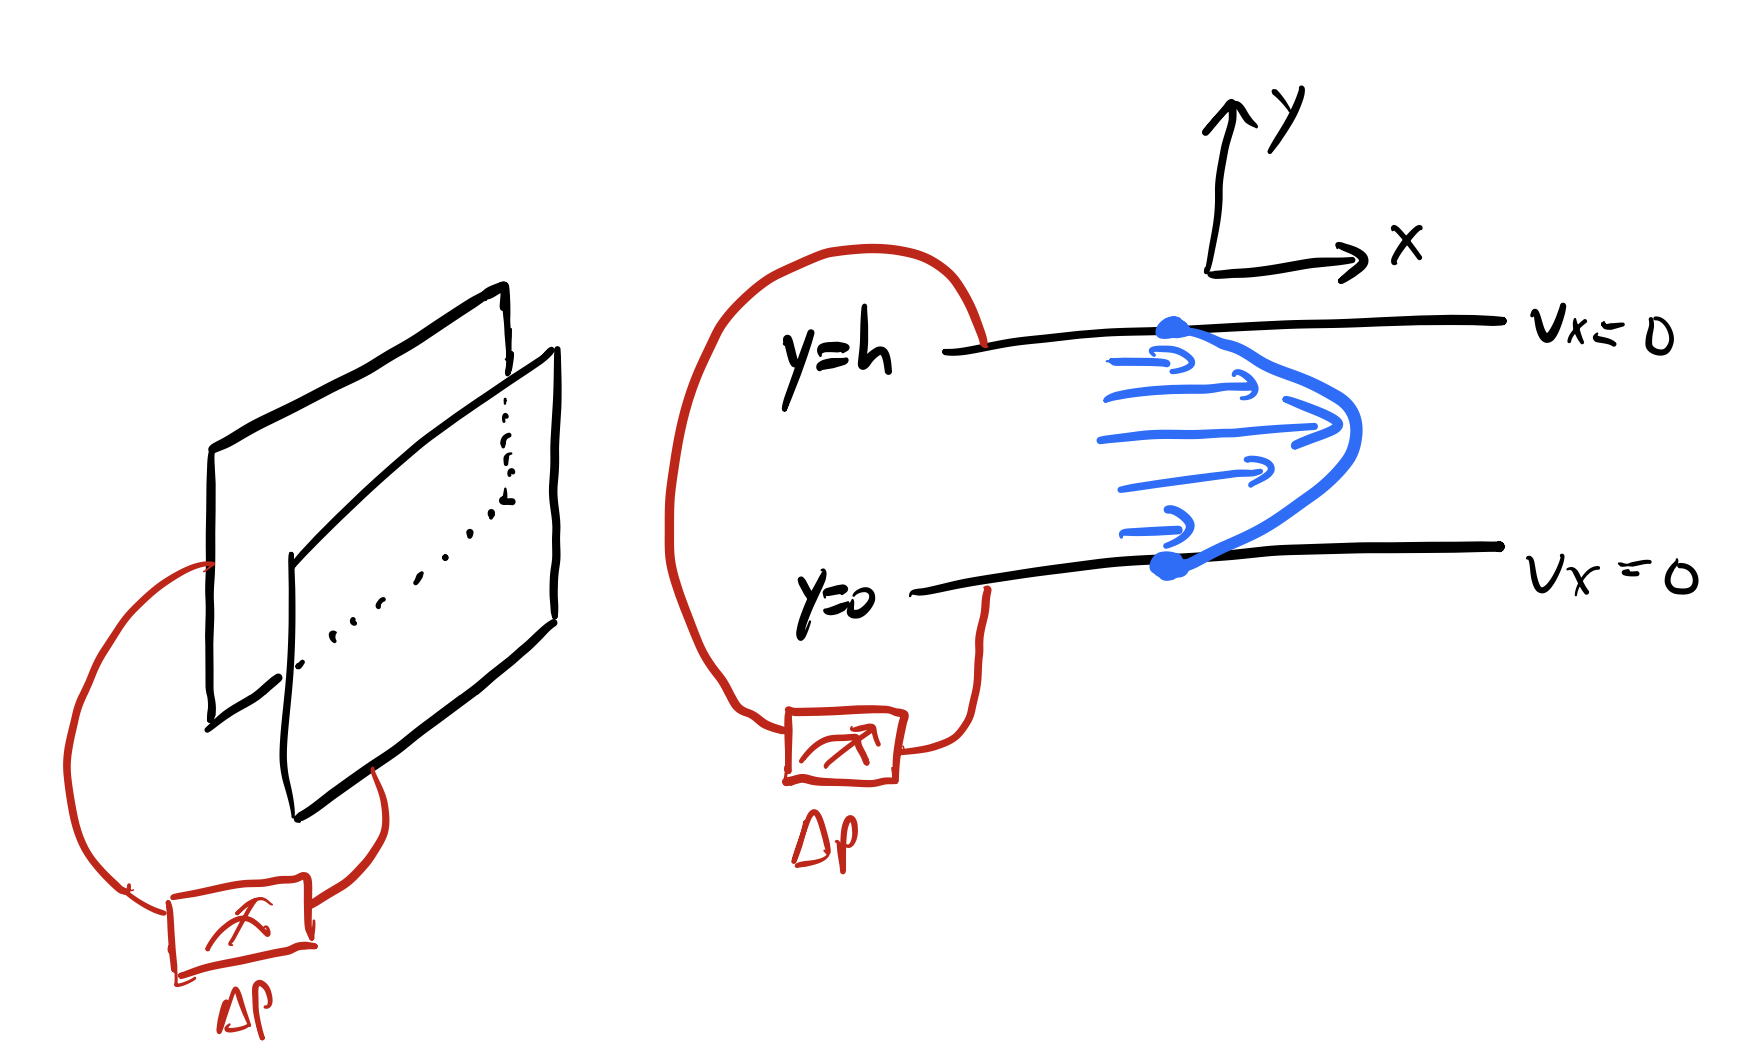
\includegraphics[scale=0.35]{Lectures/Images/lec10-pressuredifferential.png}
\end{center}

Note: When the Reynolds number is low, the $\rho D_t v_i$ term (which $\text{Re}$ multiplies) can be neglected, and then solving for the hydrodynamics reduces to:
\begin{equation}
    \eta\Delta v_i = \p_i p'
\end{equation}
Which is just the Laplace equation with a source term - this is one of the most well-solved problems in the universe; we have the solution:
\begin{equation}
    \v{v} = \frac{G}{2\eta}y(h-y)\xhat
\end{equation}
I.e. the flow looks like a parabola. This flow is unchanged by the addition of the odd viscosity term, because the solution only depends on the gradient in the x-direction.

Calculating the vorticity:
\begin{equation}
    \omega = \p_x v_y - \p_y v_x = \p_x(0) - \p_y\left(\frac{G}{2\eta}y(h-y)\right) = -\frac{G}{2\eta}(h - 2y)
\end{equation}

Now, we want to evaluate (using $p' = p - \eta^0 \omega$) the pressure differential:
\begin{equation}
    \Delta p = p(y=h) - p(y=0) = Gh\frac{\eta^0}{\eta}
\end{equation}
This is a measurable quantity, and this was measured in the 70s/80s in Linden.

\subsection{Compressible Systems}
What happens now if our fluid is compressible - e.g. we consider a gas flowing in a channel? What happens if we assume the nonlinear terms cannot be neglected?

To this end, we want to try to rewrite the the equation for the velocity field to get an equation for the vorticity. Multiplying Eq. \eqref{eq:modNavierStokes} by $\e_{li}\p_l$ (i.e. taking a curl of the equation) and defining the kinematic viscosity $\nu = \frac{\eta}{\rho}$ and $\nu^0 = \frac{\eta^0}{\rho}$ we find:
\begin{equation}
    \p_t \omega + \nabla \cdot (\omega \v{v}) = \nu \nabla^2 \omega + \nu^0\nabla^2(\nabla \cdot \v{v})
\end{equation}
Where the curl of the gradient of the pressure drops out, and the last term was obtained from:
\begin{equation}
    \e_{li}\p_l \e_{ij}\p_k\p_k v_j = \delta_{lj}\p_l \p_k \p_k v_j = \nabla^2 (\nabla \cdot \v{v})
\end{equation}
Note that the last term cooberates our story that if the fluid is incompressible then the odd viscosity term drops out of the viscosity. The odd viscosity acts as an additional source of vorticity which is proportional to the divergence of the velocity.


If we look at the pressure term in the Navier-Stokes equation:
\begin{equation}
    \frac{1}{\rho}\p_x p = \frac{1}{\rho}\dpd{p}{\rho}\dpd{\rho}{x}
\end{equation}
when $c < v$, i.e. the velocity is larger than the speed of sound in the fluid, then we can cause shock waves, and mathematically we can neglect the $\dpd{p}{\rho}\dpd{\rho}{x}$ term which is of order $c$. Therein the Navier-Stokes equation becomes:
\begin{equation}
    \boxed{\p_t v_x + v_x \p_x v_x = \nu \p_x^2 v_x}
\end{equation}
Which is an equation with both dissipation and nonlinearity, known as the \emph{Burges equation}. What he found was that the above equation can have stable solutions. This is surprising, because nonlinearities cause waves to break generically (experimentally confirm this by watching the sea by sipping a cocktail). But the diffusive/dissipative term allows for the stabilization of the nonlinearity. Though it does not appear in the above, another option would be to add dispersion (which leads to higher order equations - relevant for shallow water, for example). The stable solutions look like shock waves:

\begin{center}
    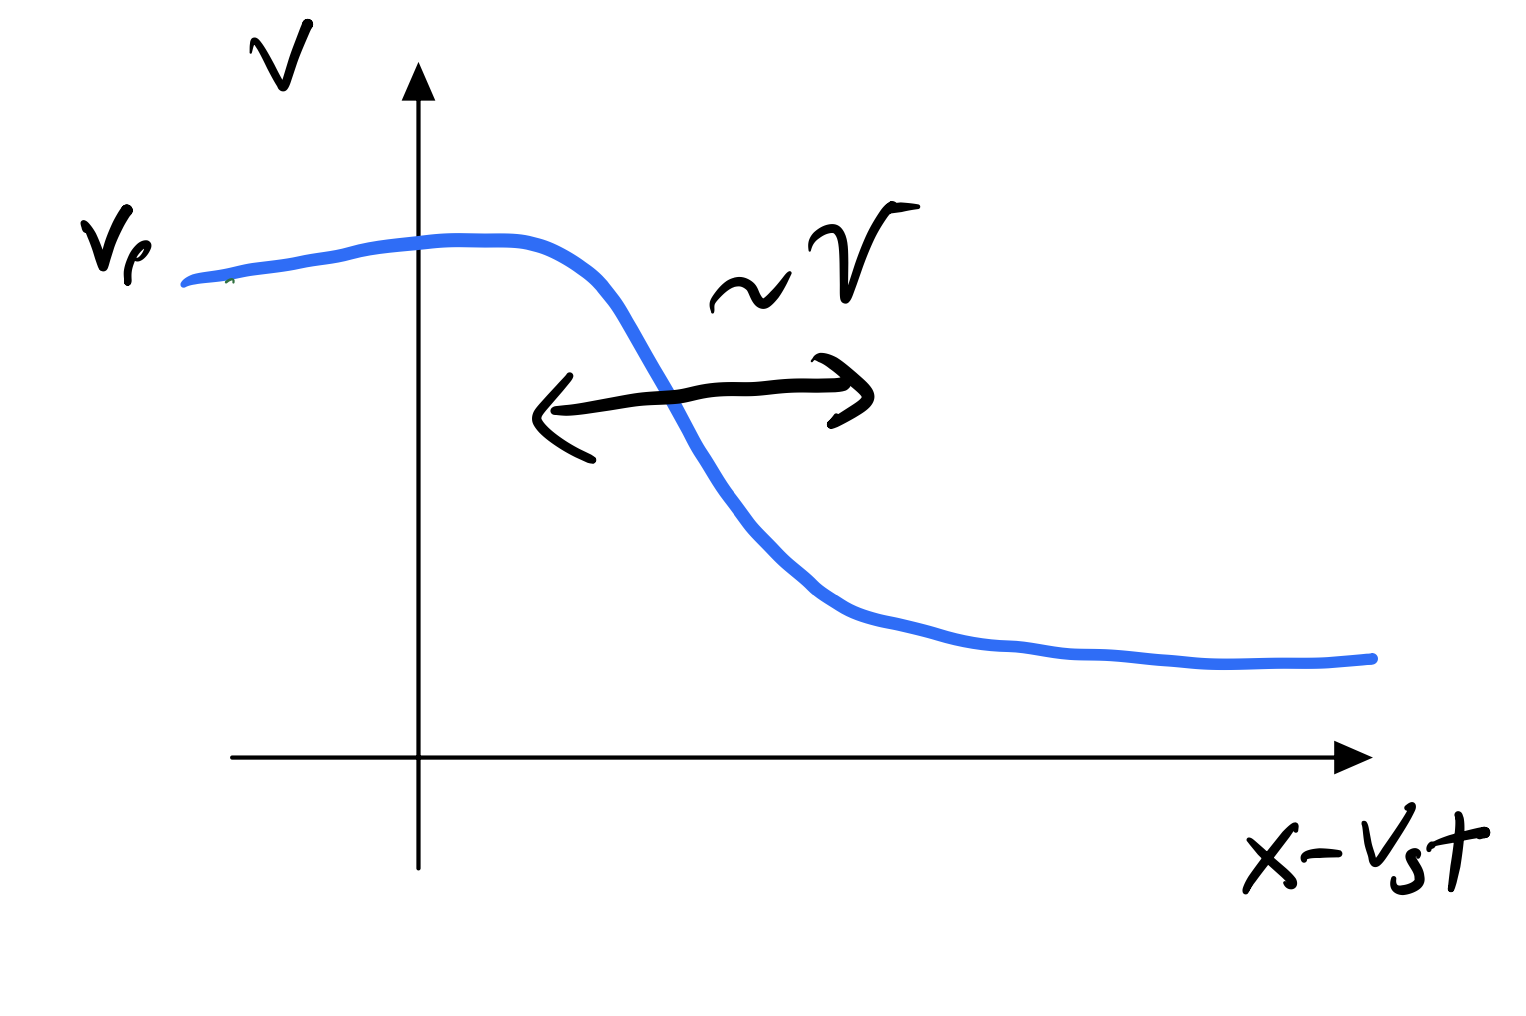
\includegraphics[scale=0.35]{Lectures/Images/lec10-shockwave.png}
\end{center}

Wherein we have a shock wave, caused by, for example, a piston moving with speed $v_p$, causing a shock wave travelling with speed $v_s$ and with width profile $\omega \sim \nu$. What happens if we calculate the divergence of the velocity? Behind and in front of the travelling shockwave wavefront, the divergence vanish. There is high concentration of divergence of velocity at the shock wavefront itself. If we now allow for flow in two dimensions, this divergence can be a source for the vorticity (we require 2D as $\omega$ is the curl of the velocity field).

You might have asked - should we not have calculated the correction to the Burges equation due to the odd viscosity. Really, we should consider:
\begin{equation}
    v_x = (\text{zeroth order}) + \frac{\eta_0}{\eta}(...)
\end{equation}
\begin{equation}
    v_y = \frac{\eta_0}{\eta}(...)
\end{equation}
The play is to calculate the zeroth order $v_x$ term, then plug things back in to calculate the first order corrections, and so on\dots But we could also be interested in the $\frac{\eta_0}{\eta} \gg 1$ limit. What happens here? Well, this corresponds to the large-odd viscosity limit. This leads to an oscillatory part/ringing of the waveform superimposed on top of the shock wave:

\begin{center}
    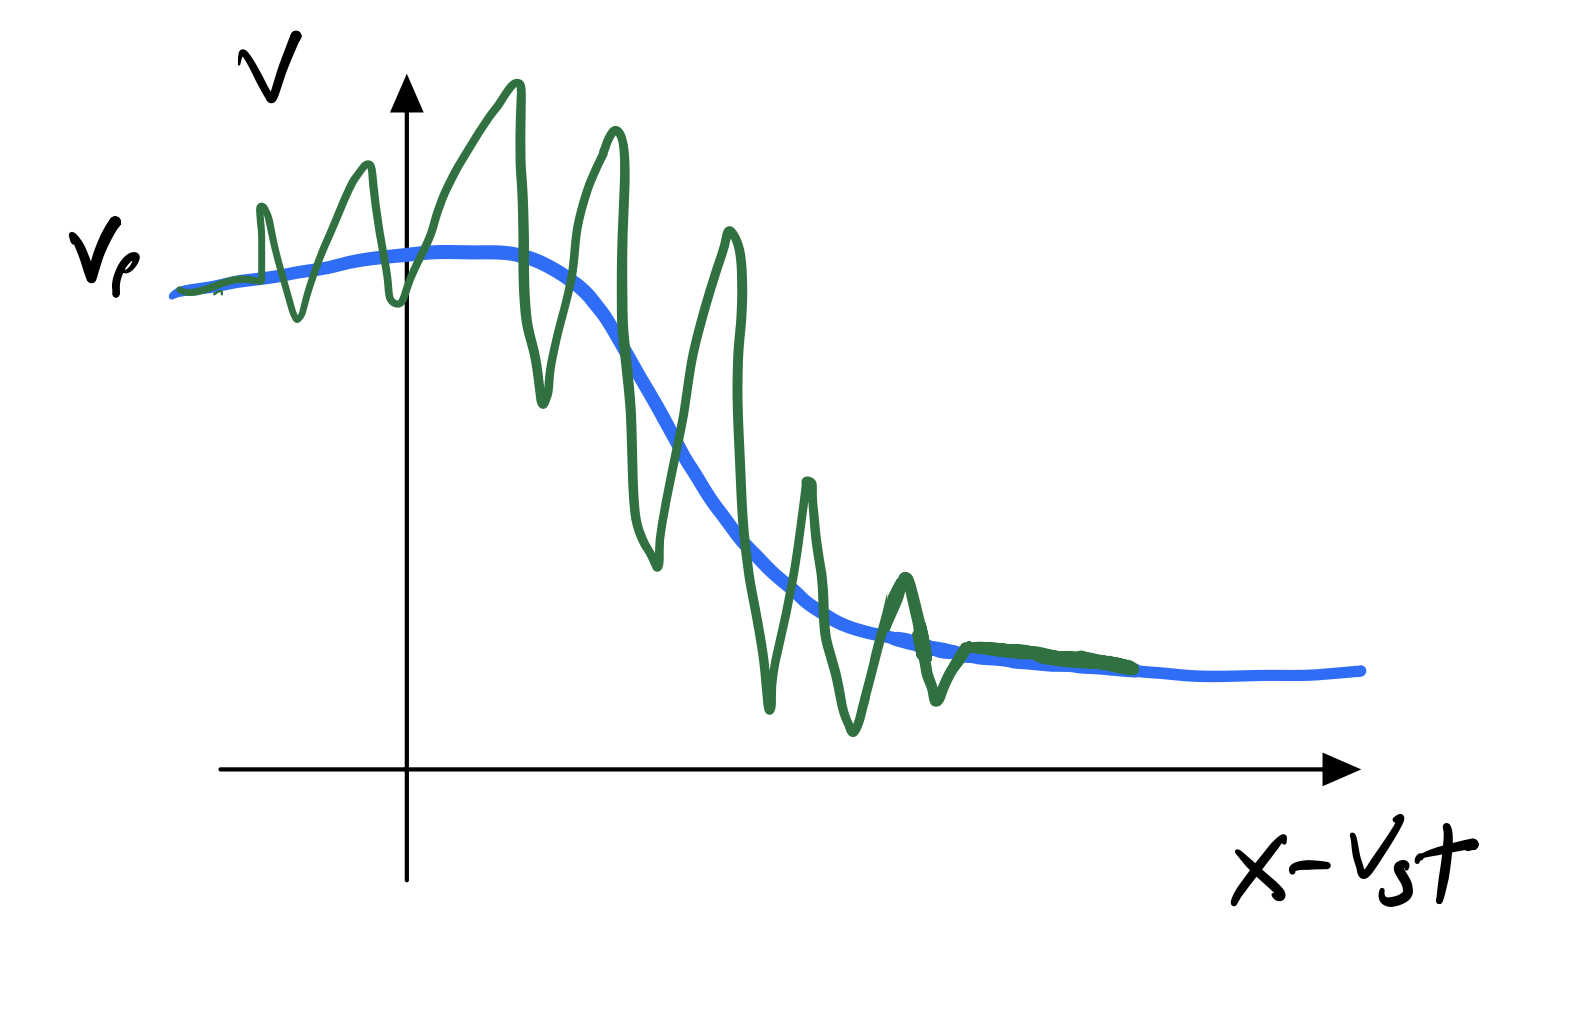
\includegraphics[scale=0.35]{Lectures/Images/lec10-ringing.png}
\end{center}

Next week, we start to discuss turbulence.